\documentclass[a4paper,11pt]{article}
\input{/home/tof/Documents/Cozy/latex-include/preambule_lua.tex}
\newcommand{\showprof}{show them}  % comment this line if you don't want to see todo environment
\fancyhead[L]{Exercices ABR}
\newdate{madate}{10}{09}{2020}
%\fancyhead[R]{\displaydate{madate}} %\today
%\fancyhead[R]{Seconde - SNT}
%\fancyhead[R]{Première - NSI}
\fancyhead[R]{Terminale - NSI}
\fancyfoot[L]{\vspace{1mm}Christophe Viroulaud}
\AtEndDocument{\label{lastpage}}
\fancyfoot[C]{\textbf{Page \thepage/\pageref{lastpage}}}
\fancyfoot[R]{\includegraphics[width=2cm,align=t]{/home/tof/Documents/Cozy/latex-include/cc.png}}

\begin{document}
\begin{commentprof}
\textbf{correction-exo-abr.zip} sur site
\end{commentprof}
\begin{exo}
    \begin{tabular}{ccccc}
        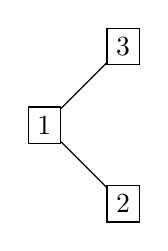
\begin{tikzpicture}
            \node[draw] (1) at (-1,-1) {1};
            \node[draw] (2) at (0,-2) {2};
            \node[draw] (3) at (0,0) {3};

            \draw (1) -- (2);
            \draw (3) -- (1);
        \end{tikzpicture}
         & 
         \begin{tikzpicture}
            \node[draw] (1) at (-2,-2) {1};
            \node[draw] (2) at (-1,-1) {2};
            \node[draw] (3) at (0,0) {3};

            \draw (1) -- (2);
            \draw (3) -- (2);
        \end{tikzpicture}
         &  
         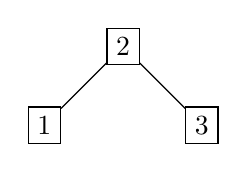
\begin{tikzpicture}
            \node[draw] (1) at (-1,-1) {1};
            \node[draw] (2) at (0,0) {2};
            \node[draw] (3) at (1,-1) {3};

            \draw (1) -- (2);
            \draw (3) -- (2);
        \end{tikzpicture}
         &  
         \begin{tikzpicture}
            \node[draw] (1) at (0,0) {1};
            \node[draw] (2) at (1,-1) {2};
            \node[draw] (3) at (2,-2) {3};

            \draw (1) -- (2);
            \draw (3) -- (2);
        \end{tikzpicture}
         &
         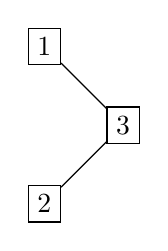
\begin{tikzpicture}
            \node[draw] (1) at (0,0) {1};
            \node[draw] (2) at (0,-2) {2};
            \node[draw] (3) at (1,-1) {3};

            \draw (1) -- (3);
            \draw (3) -- (2);
        \end{tikzpicture}
    \end{tabular}

\end{exo}
\begin{exo}
    \begin{center}
        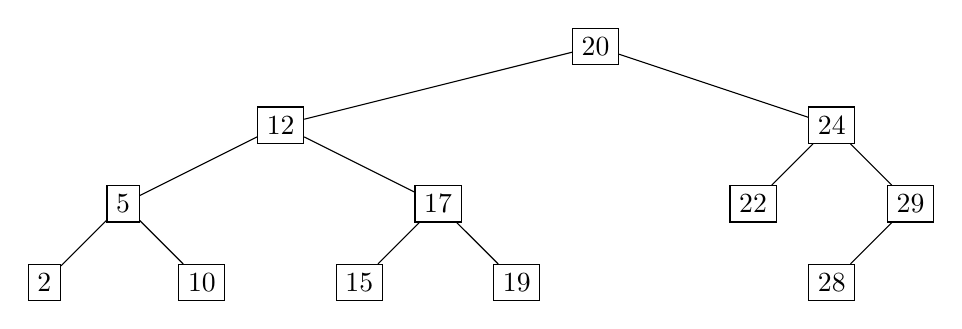
\begin{tikzpicture}
            \node[draw] (A) at (1,0) {20};
            \node[draw] (B) at (-3,-1) {12};
            \node[draw] (C) at (-5,-2) {5};
            \node[draw] (D) at (-1,-2) {17};
            \node[draw] (F) at (-4,-3) {10};
            \node[draw] (H) at (0,-3) {19};
            \node[draw] (I) at (4,-1) {24};
            \node[draw] (J) at (3,-2) {22};
            \node[draw] (K) at (-6,-3) {2};
            \node[draw] (L) at (-2,-3) {15};
            \node[draw] (M) at (5,-2) {29};
            \node[draw] (N) at (4,-3) {28};

            \draw (A) -- (B);
            \draw (C) -- (B);
            \draw (C) -- (F);
            \draw (D) -- (B);
            \draw (D) -- (H);
            \draw (A) -- (I);
            \draw (J) -- (I);
            \draw (K) -- (C);
            \draw (L) -- (D);
            \draw (M) -- (I);
            \draw (M) -- (N);
        \end{tikzpicture}
        \captionof{figure}{Un Arbre Binaire de Recherche (\emph{ABR})}
        \label{arbre}
    \end{center}
    
    [2, 5, 10, 12, 15, 17, 19, 20, 22, 24, 28, 29]
\end{exo}
\begin{exo} Retrouver la correction sur le site \url{https://cviroulaud.github.io} .
\end{exo}
\begin{exo} Retrouver la correction sur le site \url{https://cviroulaud.github.io} .

    Si l'arbre est équilibré, l'insertion de chaque élément a une complexité proportionnelle à la hauteur de l'arbre soit $O(\log(n))$ dans le pire des cas. Donc la complexité de construction de l'arbre est $O(n.\log(n))$. La recherche de l'élément est en $O(\log(n))$. Donc une complexité totale en $$O(n.\log(n) + \log(n))\simeq O(n.\log(n))$$

    Si le tableau est déjà trié, l'ABR est un peigne:
    \begin{center}
        \begin{tikzpicture}
            \node[draw] (1) at (0,0) {1};
            \node[draw] (2) at (1,-1) {2};
            \node[draw] (3) at (2,-2) {3};

            \draw (1) -- (2);
            \draw (3) -- (2);
        \end{tikzpicture}
        \captionof{figure}{ABR à partir d'un tableau déjà trié}
    \end{center}
    La construction de l'arbre est alors quadratique et la recherche dépend de n.
\end{exo}
\end{document}